\documentclass[12pt]{matmex-diploma}
\usepackage[numbers]{natbib}
\usepackage{hyperref}
\usepackage{amsmath}
\usepackage{amssymb}
\usepackage{amsthm}
\usepackage{mathtools}
\usepackage{tikz}
\usepackage{tikz-cd}
\usepackage{subdepth}
\usepackage{indentfirst}
\usetikzlibrary{calc}
\usetikzlibrary{patterns}
\usetikzlibrary{decorations.pathreplacing}
\usepackage{tcolorbox}
\usepackage{layout}
\usepackage{enumitem}

\usepackage{fontspec}
\setmainfont{Times New Roman}
\defaultfontfeatures{Mapping=tex-text}
\newfontfamily\cyrillicfont{Times New Roman} 

\makeatletter
\newcounter{aaa}
\tikzset{
  apply/.style args={#1 except on segments #2}{postaction={
      /utils/exec={
        \@for\mattempa:=#2\do{\csdef{aaa@\mattempa}{}}
        \setcounter{aaa}{0}
      },
      decorate,decoration={show path construction,
        moveto code={},
        lineto code={
          \stepcounter{aaa}
          \ifcsdef{aaa@\theaaa}{}{
            \path[#1] (\tikzinputsegmentfirst) -- (\tikzinputsegmentlast);
          }
        },
        curveto code={
          \stepcounter{aaa}
          \ifcsdef{aaa@\theaaa}{}{
            \path [#1] (\tikzinputsegmentfirst) .. controls
            (\tikzinputsegmentsupporta) and (\tikzinputsegmentsupportb)
            ..(\tikzinputsegmentlast);
          }
        },
        closepath code={
          \stepcounter{aaa}
          \ifcsdef{aaa@\theaaa}{}{
            \path [#1] (\tikzinputsegmentfirst) -- (\tikzinputsegmentlast);
          }
        },
      },
    },
  },
}
\makeatother

\makeatletter
\newcommand*{\shifttext}[2]{%
  \settowidth{\@tempdima}{#2}%
  \makebox[\@tempdima]{\hspace*{#1}#2}%
}
\makeatother



\filltitle{ru}{
    chair              = {Математика \# --- \# царица полей},
    title              = {Линейные алгебраические группы, сходные с параболическими},
    % Здесь указывается тип работы. Возможные значения:
    %   coursework - Курсовая работа
    %   diploma - Диплом специалиста
    %   master - Диплом магистра
    %   bachelor - Диплом бакалавра
    type               = {master},
    position           = {студента},
    group              = 666,
    author             = {Машкин Эдельвейс Захарович},
    supervisorPosition = {д.\,ф.-м.\,н., профессор},
    supervisor         = {Выбегалло А.\,А.},
    reviewerPosition   = {ст. преп.},
    reviewer           = {Привалов А.\,И.},
    chairHeadPosition  = {д.\,ф.-м.\,н., профессор},
    chairHead          = {Хунта К.\,Х.},
    university         = {Санкт-Петербургский Государственный Университет},
    faculty            = {Математико-механический факультет},
%    city               = {Санкт-Петербург},
%    year               = {2013}
}

\newtheoremstyle{mystyle}%                % Name
  {}%                                     % Space above
  {}%                                     % Space below
  {}%                                     % Body font
  {}%                                     % Indent amount
  {\bfseries}%                            % Theorem head font
  {.}%                                    % Punctuation after theorem head
  { }%                                    % Space after theorem head, ' ', or \newline
  {}%                                     % Theorem head spec (can be left empty, meaning `normal')


\theoremstyle{mystyle}
\newtheorem{prop}{Утверждение}
\newtheorem{hyp}{Свойство}
\newtheorem{thm}{Теорема}
\newtheorem{lm}{Лемма}
\newtheorem{rem}{Замечание}
\newtheorem{example}{Пример}
\newtheorem{definition}{Определение}


\linespread{1.3}

\newcommand{\Z}{\mathbb{Z}}
\newcommand{\N}{\mathbb{N}}
\renewcommand{\C}{\mathbb{C}}
\renewcommand{\le}{\leqslant}
\renewcommand{\ge}{\geqslant}

\def\lacts{\curvearrowright}
\def\racts{\curvearrowleft}

\newcommand\bigzero[2]{\raisebox{#2ex-2ex}[0pt][0pt]{\shifttext{#2em}{\text{\Huge{#1}}}}}

\begin{document}

\maketitle
\tableofcontents


\newcommand\placeholder{\textcolor{red}{\textbf{\\\#\\\#\\\#}}}

\section{Введение}

\layout

Линейные алгебраические группы над кольцами изучаются \placeholder

Структурная теория алгебраических групп над кольцами \placeholder

Структурная теория и нормальное строение групп Шевалле и редуктивных групп достаточно хорошо изучена и исследуется в таких работах, как \citep{Vavilov2006}, \citep{Stepanov1993}, \citep{Golubchik1975}, \citep{Hazrat2010}, \citep{Stavrova2018}.

Интерес также представляют и нередуктивные группы.
Нормальное строение параболических поддгрупп в группах Шевалле изучается в работах \citep{Azad1990}, \citep{Roehrle1990}, \citep{Roehrle1998}, \citep{Stavrova2009}.

Однако аналогичные методы изучения нередуктивных групп могут быть применены не только к параболическим подгруппам групп Шевалле и редуктивных групп, но и к более широкому классу нередуктивных групп. В данной работе эти методы применяются для описания нормального строения групп, которые строятся на основе линейного представления редуктивной группы, и по своим свойствам сходны с параболическими подгруппами групп Шевалле.

\section{Постановка задачи}

Одной из предпосылок к постановке задачи послужила следующая проблема. \placeholder

Ортогональная группа (аналогично симплектическая, эрмитова) --- подгруппа $GL$, сохраняющая билинейную форму, которая обычно предполагается невырожденной.

Или как в работе \cite{Petrov2005} --- требования невырожденности нет, но элементарная подгруппа определяется через трансвекции Эйхлера-Зигеля-Диксона:

Если $ |u|_q = 0 $, $(u,v)_q = 0$, $|v|_q = (0, a) \dot{+} \mathfrak{L}$, то
$$ T_{uv}(a) : w \mapsto w + u \bar{1}^{-1} ((v,w)_q + a(u,v)_q) + v (u,w)_q $$

Очевидно, если билинейная форма вырожденная (в частности, если она имеет вид $B \oplus 0$), то элементарная группа, определённая таким образом, существенно меньше всей группы.

Такого вида ортогональные группы уже не будут редуктивными над тем кольцом, над которым форма вырождена. Их структура достаточно близка к структуре параболческих подгрупп в группах Шевалле, хотя они в общем случае могут не вкладываются в группы Шевалле в качестве параболических подгрупп. Это сходство послужило отправной точкой для изучения более общего класса нередуктивных групп, включающего оба случая: параболические подгруппы групп Шевалле и вырожденные ортогональные группы. Структурной теории построенного обобщения --- группам, сходным с параболическими --- и посвящена данная работа.

Как известно из работы \citep{Azad1990}, на унипотентном радикале параболической подгруппы можно ввести структуру модуля, так что на некотором его фактормодуле действует подгруппа Леви. Исходной задачей данной работы было обратить данную конструкцию, а именно исследовать структуру групп, сходных с параболическими, конструируемых явным образом из некоторого заданного представления.

\section{Определения}

Следующие три определения широко известны и приведены, например, в работах \cite{Conrad11reductivegroup}, \#, \#.

\begin{definition} 
Редуктивной $R$-группой называется линейная алгебраическая $R$-группа, не содержащая нетривиальных связных нормальных унипотентных линейных алгебраических $R$-подгрупп.
\end{definition}

\begin{definition}
Полупростой $R$-группой называется линейная алгебраическая $R$-группа, не содержащая нетривиальных связных нормальных разрешимых линейных алгебраических $R$-подгрупп.
\end{definition}

\begin{definition}
Простой $R$-группой называется линейная алгебраическая $R$-группа, не содержащая нетривиальных связных нормальных линейных алгебраических $R$-подгрупп.
\end{definition}

Известно, что всякой приведённой неприводимой системе корней $\Phi$ единственным образом соответствует односвязная аффинная групповая схема $G(\Phi,-)$ над $\Z$, называемая групповой схемой Шевалле-Демазюра (\cite{Plotkin1998}, \cite{Steinberg2016}, \cite{Chevalley1960-1961}).

Под представлением алгебраической группы $G$ над кольцом $k$ понимается гомоморфизм групповых схем $G \to \mathrm{GL}_n(k)$. Это означает, что представление над базовым кольцом индуцирует с помощью расширения скаляров представление над расширенным кольцом.

Представление (над некоторым полем $k$) называется неприводимым (в терминологии \cite{Milne2017} простым), если оно не содержит нетривиальных подпредставлений.

Неприводимые представления редуктивных групповых схем над полем представляют собой модули старшего веса (\cite{Jantzen1987}, следствие 2.7).




Пусть $G_\Z$ --- связная редуктивная групповая схема с системой корней $\Phi = \Phi_1 + \dots + \Phi_n$, где $\Phi_i$ --- приведённые неприводимые системы корней, $n \ge 1$.

Далее пусть $U_\Z$ --- неприводимое (над замкнутым полем характеристики $0$) представление, то есть конечномерный свободный модуль старшего веса $G_\Z$, $\pi:G_\Z \to GL(U_\Z)$ с рангом
\begin{equation}\label{representationrank}\mathrm{rk} \; U_\Z \ge 2 \;. \end{equation}
Тогда $U=U_\Z\otimes R$ будет представлением группы $G=G_\Z(R)$ над кольцом $R$. Так как представление является морфизмом схем, то $U$, как и $U_\Z$, будет являться свободным модулем, и в случае выбора максимального тора $T$ является (\citep{Borel1970}) прямой суммой весовых подпространств
$$U=\bigoplus_{\sigma \in \Sigma \subset X(T)} {U \cap U_\sigma} ,$$
где\\
$U_\sigma = \{x \in U_\C \; | \; ^h x = \sigma(h) x \forall h \in T \}$,\\
$\Sigma = \{\sigma \in X(T) \
; | \; U_\sigma \ne \varnothing\}$ --- множество весов представления,\\
$X(T)$ --- группа рациональных характеров тора.

\section{Основные сведения о группе $G$ и её рациональном представлении $\pi$}

\placeholder

$x_\alpha(\xi)$ --- корневые элементы группы $G$.

Перечислим их основные свойства:

\begin{itemize}
\item
Для экстремальных весов (в частности, для старшего веса $\widetilde\sigma$), весовые пространства $U_\sigma$ одномерны.
\item
Корневые элементы унипотентны (как операторы конечномерного представления $(U,\pi)$):
$$\exists n : (x_\alpha(\xi)-1)^n = 1$$
Для базисных представлений (микровесовые представления, представления на коротких корнях и присоединённые представления групп с системами корней с простыми связями, \cite{Plotkin1998}) это верно уже при $n=3$. Для микровесовых представлений это верно уже при $n=2$.
\item
Корневые элементы аддитивны по параметру:
$$x_\alpha(\xi) \; x_\alpha(\theta)  = x_\alpha(\xi+\theta)$$
$$x_\alpha(\xi)^n = x_\alpha(n \, \xi) \; \forall n \in \Z$$
\end{itemize}

На модуле $U$ корневые элементы действуют как операторы. Поэтому, eсли в базовом кольце числа $2 \ldots n-1$ обратимы, то определён логарифм корневых элементов, который является полиномиальной функцией от корневых элементов:
$$ \varepsilon_\alpha(\xi) \coloneqq \mathrm{ln} \, x_\alpha(\xi) = \sum_{i=0}^{n-1} {x_\alpha(\xi)^i k_i} $$
При этом имеется изоморфизм (над базовым кольцом) между корневыми подгруппами $\left<x_\alpha(\xi)\right>$ и циклическими группами, порождёнными $\varepsilon_\alpha(\xi)$.

Можно видеть, что умножение параметра на целое число эквивалентно умножению на число самого оператора $\varepsilon_\alpha(\xi)$:
$$ \varepsilon_\alpha(n \, \xi) = \mathrm{ln} \, x_\alpha(n \, \xi) = \mathrm{ln} \, x_\alpha(\xi)^n = n \; \mathrm{ln} \, x_\alpha(\xi) = n \; \varepsilon_\alpha(\xi) \; \forall n \in \Z
$$

Так как изоморфизм  между циклическими группами $\left<x_\alpha(\xi)\right> \le G$ и $\left<\varepsilon_\alpha(\xi)\right> \le \mathrm{GL}(U)$ определён над базовым кольцом, то аналогичным образом выглядит умножение параметра на произвольные константы:
$$
\varepsilon_\alpha(\eta \, \xi) = \eta \; \varepsilon_\alpha(\xi) \; \forall \eta \in R
$$

\begin{lm}
Оператор $\varepsilon_\alpha(\xi)$ переводит элементы из подпространства $U_\sigma$ в подпространство $U_{\sigma+\alpha}$.
\end{lm}
\begin{proof}
\begin{multline*}
^h(\varepsilon_\alpha(\xi) \, u) =
^h\left(\sum_i \, {^{x_\alpha(\xi)^i}u \, k_i}\right) = 
\sum_i \, {^{h x_\alpha(\xi)^i}u \, k_i} = \\ =
\sum_i \, {^{(^h x_\alpha(\xi))^i h}u \, k_i} = 
\sum_i \, {^{(x_\alpha(\alpha(h)\cdot\xi))^i} \left(^h u\right) \, k_i} =\\=
\sum_i \, {^{(x_\alpha(\alpha(h)\cdot\xi))^i} u \cdot \sigma(h) \, k_i} =
\varepsilon_\alpha(\alpha(h)\cdot\xi) \, u \cdot \sigma(h) = \\ =
\varepsilon_\alpha(\xi) \, u \cdot \alpha(h)\sigma(h)
\end{multline*}
\end{proof}

Следующее требование, которые мы в дальнейшем будем предполагать выполненным, относится одновременно к модулю $U$ и кольцу $R$. Для базисных представлений без нулевого веса оно выполнено всегда независимо от кольца $R$, но для более сложных случаев оно можно означать обратимость в $R$ некоторых целых чисел.

\begin{hyp}\label{returnfromhighest}
Если $u$ --- некоторый вектор из $U_\sigma$, и $V={}^{EB}\left<u\right>$ --- минимальный $EB$-инвариантный подмодуль, содержащий $u$, то $u \in {}^E\left<V \cap U_{\widetilde\sigma}\right>$, или, что то же самое, ${}^E\left<V \cap U_{\widetilde\sigma}\right> = {}^E \left<u\right>$.

Иными словами, если $u$ --- некоторый вектор из $U_\sigma$, то его образы в пространстве $U_{\widetilde\sigma}$ старшего веса под действием операторов 
$\left(\prod_{\alpha_i}\varepsilon_{\alpha_i}(1)\right)$, где $\alpha_i$ пробегает по всем цепочам положительных корней, так что $\sum_i \alpha_i = \widetilde\sigma - \sigma$, не содержатся ни в каком $E$-инвариантном модуле, в котором бы не содержался $u$. Иными словами, все эти образы в совокупности порождают (как $E$-инвариантный подмодуль) тот же самый подмодуль, который порождается (как $E$-инвариантный подмодуль) исходным вектором $u$.
\end{hyp}

Следующие утверждения вытекают из данного свойства:

\begin{lm} \label{extremalweightisomorphism}
Если $\sigma$ и $\sigma+n\alpha$ --- экстремальные корни и $u\in U_\sigma$, то
если $\varepsilon_\alpha(1)^n \, u $ содержится в некотором $E$-инвариантном подмодуле $V$, то и $u \in V$.
\end{lm}
\begin{proof}
Если $\sigma+n\alpha = \widetilde\sigma$ --- максимальный корень, то утверждение является частным случаем \ref{returnfromhighest}. В остальных случаях $\sigma+n\alpha$ переводится в $\widetilde\sigma$ некоторым элементом группы Вейля.
\end{proof}

\begin{lm}\label{weightprojections}
Если $V$ --- инвариантный подмодуль $U$, то $V = \bigoplus V_\sigma$, то есть проекции вектора $v \in V$ на корневые подпространства также лежат в $V$.
\end{lm}
\begin{proof}
Пусть $v = \sum v_\sigma$. Доказательство проведём индукцией по минимальному (то есть не имеющему меньших) весу $\sigma'$ из присутствующих в сумме. Базой индукции будет сумма из одного слагаемого старшего веса: $v = v_{\widetilde\sigma}$.

Пусть теперь $v = v_{\sigma'} + v'$, где $v'$, если лежит в $V$, то раскладывается в $V$ по весовым простраствам по индукционному предположению. Тогда цепочки положительных корней из свойства \ref{returnfromhighest} будут переводить $v$ в различные $w := \left(\prod_{\alpha}\varepsilon_\alpha(1)\right) \, v \in V \cap U_{\widetilde\sigma}$. Но одновременно каждый такой $w = \left(\prod_{\alpha}\varepsilon_\alpha(1)\right) \, v_{\sigma'}$, поэтому, в силу \ref{returnfromhighest}, $v_{\sigma'}$ также лежит в $V$.
\end{proof}

\begin{lm}\label{unipotentsubgroups}
Над кольцами, для которых выполняется (\ref{returnfromhighest}), инвариантные подмодули $U$ имеют вид $U_I = U \cdot I$, где $I \trianglelefteq R$.
\end{lm}
\begin{proof}
Пусть $V$ --- инвариантный подмодуль $U$. Достаточно доказать, что найдётся идеал $I$, такой что любой $V \cap U_\sigma = U_\sigma \, I$.

Cвойство \ref{returnfromhighest} устанавливает набор отображений, однозначно определяющих $V \cap U_{\widetilde\sigma}$ по $V \cap U_\sigma$ и наоборот. В силу одномерности $U_{\widetilde\sigma}$ подмодуль $V \cap U_{\widetilde\sigma}$ имеет вид $U_{\widetilde\sigma} \, I$ для некоторого идеала $I$. Следовательно, подмодули $U_{\sigma} \, I$ совпадают с $V \cap U_\sigma$.
\end{proof}

Есть предположение, что утверждение \ref{unipotentsubgroups} эквивалентно свойству \ref{returnfromhighest}. Однако доказать это предположение пока не удаётся, так как для этого нужно доказать, что ${}^EB\left<u\right> \cap U_{\widetilde\sigma} = {}^E\left<u\right> \cap U_{\widetilde\sigma}$.


\section{Элементарная группа}

Аддитивную группу $R[G]$-модуля $U$ можно рассматривать как абелеву группу с действием $G$ на ней, поэтому
имеет смысл полупрямое произведение $$P := G \rightthreetimes U.$$

Это делает логичным использование мультипликативной нотации для обозначения сложения в $U$, а также обозначение действия $G$ на $U$ через $$^{g}u = g u g^{-1}.$$ 

Обозначим за $E = E(\Phi,R)$ подгруппу в $G$, порождённую корневыми унипотентами $x_\alpha(\xi)$, где $\alpha \in \Phi$, $\xi \in R$.

Сформулируем несколько простых свойств коммутаторов в $G \rightthreetimes U$:

\begin{itemize}[label={\LARGE\raisebox{-0.5ex}{\textbullet}\quad},leftmargin=4\parindent]
\item
$[[g,u],v] = 1, \quad g \in G, \ u,v \in U $
\linespread{3}
\item 
$[g,uv] = [g,u][g,v], \quad g \in G, \ u,v \in U $
\item
$[g,hu] = [g,h]\cdot{}^h[g,u], \quad g,h \in G, \ u \in U $
\item
$[g,{}^{h}u] = {}^h[\;{}^{h^{-1}}g\,,u], \quad g,h \in G, \ u \in U $
\end{itemize}


\section{Вспомогательные утверждения}

\begin{lm}(\citep{Stavrova2009}, Theorem 2.3, Corollary 2.4)
  \label{directproduct}
  Пусть $G = G(\Phi, R)$ --- редуктивная групповая схема Шевалле-Демазюра
  с системой корней $\Phi = \Phi_1 + \ldots + \Phi_n$, где каждая неприводимая система корней $\Phi_i$ имеет ранг не меньше $2$. В коммутативном кольце $R$ предполагается обратимость всех необходимых структурных констант.
  
  Тогда если подгруппа $H \le G$ нормализуется элементарной группой $E = E(\Phi,R)$, то её коммутант с $E$ можно записать в виде прямого произведения
  $$ [H, E] = \prod_{i=1}^n E(\Phi_i,R,I_i), $$
  где $E(\Phi_i,R,I_i) = E(\Phi_i,I_i)^{E(\Phi_i,R)}$, $I_i \trianglelefteq R$
\end{lm}

\begin{lm}(\citep{Stavrova2009}, Lemma 4.2)
  \label{transitivity}
  Для любых двух корней $\alpha, \beta \in \Phi$, таких что их сумма также является корнем, и для любых  $\xi \in R$, $I \trianglelefteq R$ выполнено
  $$ \left< x_\alpha(\xi) \right>^{X_\beta(I)} \ge X_{\alpha + \beta}(\xi I), $$  
  где $X_\alpha(I) = \{x_\alpha(\xi) | \xi \in I\}$ --- относительная корневая подгруппа в $G$. Запись $\left<F\right>^H$ обозначает наименьшую подгруппу, нормализуемую $H$ и содержащую $F$, то есть подгруппу, порождённую всевозможными сопряжениями $^hf$, $f \in F$, $h \in H$.
\end{lm}

\begin{lm} \label{maximalgenerates}
  В группе Шевалле $G=G(\Phi,R)$ с неприводимой системой корней $\Phi$ с рангом $\mathrm{rk}\Phi \le 2$ выполнено
  $$X_{\widetilde\beta}(I)^{E(\Phi,R)} = E(\Phi,R,I),$$
  где $\widetilde\beta$ --- максимальный корень в $\Phi$.
\end{lm}
\begin{proof}
  Очевидно, что
\begin{align*}
  X_{\widetilde\beta}(I) &\le E(\Phi,I) \\
  X_{\widetilde\beta}(I)^{E(\Phi,R)} &\le E(\Phi,I)^{E(\Phi,R)} = E(\Phi,R,I)
\end{align*}
  Обратное включение вытекает из леммы \ref{transitivity}.
  
  Действительно, возьмём в лемме \ref{transitivity} в качестве $\alpha$ максимальный корень $\widetilde{\beta}$, а в качестве идеала $I$ всё кольцо $R$. Тогда
  $$ \left< x_{\widetilde\beta}(\xi) \right>^{X_\beta(R)} \ge X_{\widetilde\beta + \beta}(\xi R). $$
  Но так как любой корень из $\Phi$ может быть получен прибавлением к максимальному корню $\widetilde\beta$ некоторого отрицательного корня $\beta \in \Phi^-$, то группа $E(\Phi,I)$ порождается подгруппами $X_{\widetilde\beta + \beta}(I)$, а следовательно 
\begin{align*}
E(\Phi,I) &\le \left< X_{\widetilde\beta}(I) \right>^{E(\Phi,R)}\\
  E(\Phi,R,I) = E(\Phi,I)^{E(\Phi,R)} &\le \left< X_{\widetilde\beta}(I) \right>^{E(\Phi,R)}
\end{align*}
\end{proof}


\begin{lm}\label{unipotenttransitivity}
  Любая подгруппа $H \le U$, нормализуемая $G$, имеет вид $U_I$, где $I$ --- идеал кольца.
\end{lm}
\begin{proof}
  Данное утверждение является мультипликативной записью утверждения \ref{unipotentsubgroups}.
\end{proof}


\begin{lm}\label{maxrootsum}
Пусть $\Phi=\Phi_1+\ldots+\Phi_n$ --- система корней с неприводимыми компонентами ранга не менее $2$, $\widetilde\beta_1 \ldots \widetilde\beta_n$ ---  максимальные корни в неприводимых компонентах, $\sigma$ --- некоторый доминантный вес, такой что каждая разность $\sigma-\widetilde\beta_i$ не ортогональна $\Phi_i$.

Тогда каждый максимальный корень $\widetilde\beta_i$ можно представить в виде суммы двух корней $\gamma$ и $\delta$ одинаковой длины, так что любая положительная комбинация корней $\widetilde\beta_i$ и $-\gamma$ будет неотрицательна. Если же $\langle\sigma-\widetilde\beta_i,\widetilde\beta_i\rangle=0$, то выбор можно совершить таким образом, чтобы дополнительно выполнялось $\langle\sigma,\delta-\gamma\rangle>0$.

Заметим, что угол между $\gamma$ и $\delta$ в результате может оказаться либо $\frac{\pi}{2}$, либо $\frac{2\pi}{3}$. Угол $\frac{\pi}{3}$ (когда $\Phi_i = \mathrm{G}_2$) невозможен, так как тогда нарушится условие $\N\widetilde\beta_i-\N\gamma \nprec 0$.
\end{lm}
\begin{proof}
При $\Phi_i=\mathrm{G}_2$ требованиям леммы удовлетворяет выбор $\gamma=\alpha_2$ и $\delta=3\alpha_1+\alpha_2$.

\begin{center}
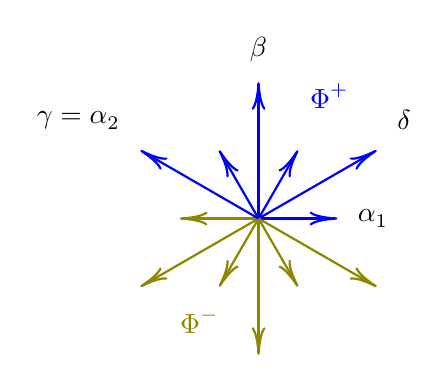
\begin{tikzpicture}[thick, scale=1]
\foreach\ang in {0,60,120}{
  \draw[blue,-{>[length=10,width=5]}] (0,0) -- ++(\ang:1);
  \draw[blue,-{>[length=10,width=5]}] (0,0) -- ++(\ang+30:{sqrt(3)});
  \draw[olive,-{>[length=10,width=5]}] (0,0) -- ++(\ang+180:1);
  \draw[olive,-{>[length=10,width=5]}] (0,0) -- ++(\ang+180+30:{sqrt(3)});
}
\path (0,0) ++(0:1) node [label=right:$\alpha_1$] {};
\path (0,0) ++(150:{sqrt(3)}) node [label=above left:{$\gamma=\alpha_2$}] {};
\path (0,0) ++(90:{sqrt(3)}) node [label=above:$\beta$] {};
\path (0,0) ++(30:{sqrt(3)}) node [label=above right:$\delta$] {};
\node[blue] at (60:1.8) {$\Phi^+$};
\node[olive] at (180+60:1.5) {$\Phi^-$};
\end{tikzpicture}
\end{center}

Пусть теперь $\Phi_i\ne\mathrm{G}_2$. Условие $k\widetilde\beta_i-l\gamma\nprec 0\;\forall k,l\in\N$ выполняется автоматически, если угол между $\gamma$ и $\delta$ составляет $\frac{2\pi}{3}$. Если же угол $\frac{\pi}{2}$, то обеспечить выполнения этого условия можно заменой местами $\gamma$ и $\delta$, чтобы $\delta-\gamma>0$.

\begin{center}
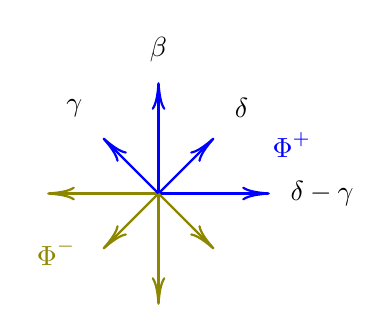
\begin{tikzpicture}[thick, scale=1]
\foreach\ang in {0,90}{
  \draw[blue,-{>[length=10,width=5]}] (0,0) -- ++(\ang:{sqrt(2)});
  \draw[blue,-{>[length=10,width=5]}] (0,0) -- ++(\ang+45:1);
  \draw[olive,-{>[length=10,width=5]}] (0,0) -- ++(\ang+180:{sqrt(2)});
  \draw[olive,-{>[length=10,width=5]}] (0,0) -- ++(\ang+180+45:1);
}
\path (0,0) ++(0:{sqrt(2)}) node [label=right:$\delta-\gamma$] {};
\path (0,0) ++(90+45:1) node [label=above left:{$\gamma$}] {};
\path (0,0) ++(90:{sqrt(2)}) node [label=above:$\beta$] {};
\path (0,0) ++(45:1) node [label=above right:$\delta$] {};
\node[blue] at (20:1.8) {$\Phi^+$};
\node[olive] at (180+30:1.5) {$\Phi^-$};
\end{tikzpicture}
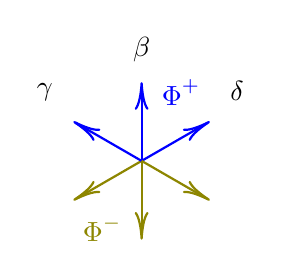
\begin{tikzpicture}[thick, scale=1]
\foreach\ang in {0,60,120}{
  \draw[blue,-{>[length=10,width=5]}] (0,0) -- ++(\ang+30:1);
  \draw[olive,-{>[length=10,width=5]}] (0,0) -- ++(\ang+180+30:1);
}
\path (0,0) ++(150:1) node [label=above left:{$\gamma$}] {};
\path (0,0) ++(90:1) node [label=above:$\beta$] {};
\path (0,0) ++(30:1) node [label=above right:$\delta$] {};
\node[blue] at (60:1) {$\Phi^+$};
\node[olive] at (180+60:1) {$\Phi^-$};
\end{tikzpicture}
\end{center}

В случае, когда $\langle\sigma-\widetilde\beta_i,\widetilde\beta_i\rangle=0$, обеспечить выполнения условия $\langle\sigma,\delta-\gamma\rangle>0$ можно следующим образом. Выберем корень $\delta$, не ортогональный ни $\widetilde\beta_i$, ни $\sigma-\widetilde\beta_i$ (это можно сделать, так как $\Phi$ неприводима и в $\Phi$ есть корень, не ортогональный $\sigma-\widetilde\beta_i$). Не умаляя общности можно считать, что $\langle\delta,\widetilde\beta_i\rangle>0$ и $\langle\delta,\sigma-\widetilde\beta_i\rangle>0$. Тогда $\langle\delta,\widetilde\beta_i\rangle=\frac{1}{2}\langle\widetilde\beta_i,\widetilde\beta_i\rangle$ и $\gamma\coloneqq\widetilde\beta_i-\delta$. При этом
$\langle\sigma,\delta-\gamma\rangle =
\langle\sigma,2\delta-\widetilde\beta_i\rangle =
2\langle\sigma,\delta\rangle-\langle\sigma,\widetilde\beta_i\rangle = 
2\langle\sigma,\delta\rangle-\langle\widetilde\beta_i,\widetilde\beta_i\rangle =
2\langle\delta,\sigma\rangle-2\langle\delta,\widetilde\beta_i\rangle =
2\langle\delta,\sigma-\widetilde\beta_i\rangle > 0$.
Условие $k\widetilde\beta_i-l\gamma\nprec 0\;\forall k,l\in\N$ при этом будет выполнено, так как  $\delta-\gamma$ не может быть отрицательным корнем (если это корень, то положительный).
\end{proof}

\begin{lm}\label{highestweightvariants}
При выборе $\gamma$ и $\delta$ согласно предыдущей лемме выполняется хотя бы одно из следующих условий:
\begin{itemize}
\item Если угол между $\gamma$ и $\delta$ составляет $\frac{2\pi}{3}$:
\begin{enumerate}
\item $ \sigma - \gamma \notin \Sigma$
\item $ \sigma - \delta \notin \Sigma$
\item $ \sigma - 2\gamma \in \Sigma$
\item $ \sigma - 2\delta \in \Sigma$
\end{enumerate}
\item Если угол между $\gamma$ и $\delta$ составляет $\frac{\pi}{2}$:
\begin{enumerate}
\item[0.] $ \sigma - \delta + \gamma \in \Sigma$
\item $ \sigma - 2\gamma \notin \Sigma$
\item $ \sigma - 2\delta \notin \Sigma$
\item $ \sigma - 3\gamma \in \Sigma$
\item $ \sigma - 3\delta \in \Sigma$
\end{enumerate}
\end{itemize}
\end{lm}

\begin{proof}
Очевидно что,
$$ \sigma - \frac{2 \langle \sigma,\gamma\rangle}{\langle \gamma , \gamma \rangle}\gamma \;\in\; \Sigma $$
$$ \sigma - \frac{2 \langle \sigma,\delta\rangle}{\langle \delta , \delta \rangle}\delta \;\in\; \Sigma \; , $$
но при этом
$$ \sigma - \frac{2 \langle \sigma,\gamma\rangle}{\langle \gamma , \gamma \rangle}\gamma-\gamma \;\notin\; \Sigma $$
$$ \sigma - \frac{2 \langle \sigma,\delta\rangle}{\langle \delta , \delta \rangle}\delta-\delta \;\notin\; \Sigma \; . $$
Следовательно, условия (1-4) могут выполняться, только если $\langle\sigma,\gamma\rangle=\langle\widetilde\beta_i,\gamma\rangle$
и одновременно $\langle\sigma,\delta\rangle=\langle\widetilde\beta_i,\delta\rangle$. Но это значит, что $\langle\sigma-\widetilde\beta_i,\widetilde\beta_i\rangle=0$,
а значит по предыдущей лемме $\langle\sigma,\delta-\gamma\rangle > 0$, то есть выполнено условие (0).
\end{proof}

\section{Основной результат}

Теперь, можно перейти к описанию подгрупп в $P=G\rightthreetimes U$, нормализуемых элементарной группой $E\le G$.

\begin{thm}\label{subgroupprojectionmain}
  Снова $G = G(\Phi, R)$ --- редуктивная групповая схема Шевалле-Демазюра
  с системой корней $\Phi = \Phi_1 + \ldots + \Phi_n$, где каждая $\Phi_i$ --- неприводимая система корней ранга не меньше $2$. $U$ --- неприводимое рациональное представление $G$ (модуль Вейля) с таким старшим весом $\widetilde\sigma$, что ни для какой неприводимой компоненты $\Phi_i$ с максимальным весом $\widetilde\beta_i$ не оказывается $\widetilde\sigma-\widetilde\beta_i$ ортогональным всей $\Phi_i$. В коммутативном кольце $R$ предполагается обратимость всех структурных констант группы $G$, а также предполагается выполнение свойства \ref{returnfromhighest}.
    
  Пусть имеется подгруппа $H \le G \rightthreetimes U$, нормализуемая группой $E$, то есть $[H,E] \le H$. Тогда образ $H$ при проекции $G \rightthreetimes U \rightarrow G$, обозначаемый как $H_G$, будет обладать следующим свойством: $[H_G,E]\le H$.
\end{thm}
\begin{proof}
  $H$ нормализуется $E$, следовательно $H_G$ также нормализуется $E$. По лемме \ref{directproduct} $[H_G,E] = \prod_{i=1}^n E(\Phi_i,R,I_i)$ при некотором выборе идеалов $I_i$. Требуется доказать, что $[H_G,E] \le H$, то есть в прямом произведении $\prod_{i=1}^n E(\Phi_i,R,I_i)$ каждый множитель $E(\Phi_i,R,I_i)$  лежит в $H$.

Но по лемме \ref{maximalgenerates} $E(\Phi_i,R,I_i) = X_{\widetilde\beta_i}(I_i)^{E(\Phi_i,R)}$.

Поэтому достаточно доказать, что $X_{\widetilde\beta_i}(I_i)^{E(\Phi_i,R)} \le H$, то есть что
$x_{\widetilde{\beta_i}}(\xi) \in H \ \forall \xi \in I_i$.

По построению известно, что $x_{\widetilde\beta_i}(\xi) \in [H_G,E] \le H_G$.
Обозначим за $h$ некоторый прообраз $x_{\widetilde\beta_i}(\xi)$ при проекции $G \rightthreetimes U \rightarrow G$.

\begin{equation*}
\tikzset{
  Subgroup/.style={
    draw=none,
    every to/.append style={
      edge node={node [sloped, allow upside down, auto=false]{$\le$}}}},
  Equals/.style={
    draw=none,
    every to/.append style={
      edge node={node [sloped, allow upside down, auto=false]{$=$}}}},
  Included/.style={
    draw=none,
    every to/.append style={
      edge node={node [sloped, allow upside down, auto=false]{$\in$}}}}
}
\begin{tikzcd}
G \rightthreetimes U \arrow{r}{} & G \\
H \arrow[Subgroup]{u} \arrow{r}{} & H_G \arrow[Subgroup]{u} \\
h \arrow[Included]{u} \arrow[maps to]{r}{} & x_{\widetilde\beta_i}(\xi) \arrow[Included]{u} \\
x_{\widetilde\beta_i}(\xi)\,u \arrow[Equals]{u} \arrow[maps to]{r}{} & x_{\widetilde\beta_i}(\xi) \arrow[Equals]{u} \\
\end{tikzcd}
\end{equation*}

Рассмотрим два случая. Пусть сначала $u \notin U_{\widetilde\sigma}$, то есть $u$ не является вектором максимального веса.
Разложим $u$ по весовым подпространствам: $$u = \prod_{\sigma \in \Sigma} u_\sigma = u_{\widetilde\sigma} \, \prod_{\sigma \in \Sigma \setminus \{\widetilde\sigma\} } u_\sigma = u_{\widetilde\sigma} \, u'  .$$
Докажем, что все множители, составляющие $u'$, принадлежат $H$. Будем доказывать это по индукции по аналогии с леммой \ref{weightprojections}.

Пусть $\sigma$ --- минимальный корень из присутствующих в разложении $u'$. Для некоторого положительного корня $\alpha_1 \in \Phi$ (не обязательно из $\Phi_i$) вычислим
\begin{multline*}
[x_{\alpha_1}(1), h] = [x_{\alpha_1}(1), x_{\widetilde\beta_i}(\xi)u] =
[x_{\alpha_1}(1), x_{\widetilde\beta_i}(\xi)] \cdot {}^{x_{\widetilde\beta_i}(\xi)}[x_{\alpha_1}(1),u] =\\=
{}^{x_{\widetilde\beta_i}(\xi)}[x_{\alpha_1}(1),u] \; \in \; U \cap H \; .
\end{multline*}

Рассмотрим цепочку положительных корней $\alpha_1,\alpha_2 \ldots \alpha_k$, начинающуюся с $\alpha_1$, такую что $\alpha_1+\alpha_2+\ldots+\alpha_k=\widetilde\sigma-\sigma$. Последовательное коммутирование $u_\sigma$ с корневыми элементами этой цепочки приводит к такому же результату, как действие оператора $\varepsilon_{\alpha_k}(1)\ldots\varepsilon_{\alpha_2}(1)\varepsilon_{\alpha_1}(1)$:
$$ [x_{\alpha_k}(1),[\ldots[x_{\alpha_2}(1),[x_{\alpha_1}(1),u_\sigma]]\ldots]] =
\big(\varepsilon_{\alpha_k}(1)\ldots\varepsilon_{\alpha_2}(1)\varepsilon_{\alpha_1}(1)\big)(u_\sigma) \;.$$
При этом к тому же результату приводит и аналогичное коммутирование $u$
$$ [x_{\alpha_k}(1),[\ldots[x_{\alpha_2}(1),[x_{\alpha_1}(1),u]]\ldots]] =
\big(\varepsilon_{\alpha_k}(1)\ldots\varepsilon_{\alpha_2}(1)\varepsilon_{\alpha_1}(1)\big)(u_\sigma) \;,$$
а также коммутирование $h$:
\begin{multline*}
[x_{\alpha_k}(1),[\ldots[x_{\alpha_2}(1),[x_{\alpha_1}(1),h]]\ldots]] =\\=
[x_{\alpha_k}(1),[\ldots[x_{\alpha_2}(1),{}^{x_{\widetilde\beta_i}(\xi)}[x_{\alpha_1}(1),u]]\ldots]] =\\=
[x_{\alpha_k}(1),[\ldots{}^{x_{\widetilde\beta_i}(\xi)}[x_{\alpha_2}(1),[x_{\alpha_1}(1),u]]\ldots]] =\\=
{}^{x_{\widetilde\beta_i}(\xi)}[x_{\alpha_k}(1),[\ldots[x_{\alpha_2}(1),[x_{\alpha_1}(1),u]]\ldots]] =\\=
\big(\varepsilon_{\alpha_k}(1)\ldots\varepsilon_{\alpha_2}(1)\varepsilon_{\alpha_1}(1)\big)(u_\sigma) \;,
\end{multline*}

В результате по свойству \ref{returnfromhighest}, так как $\big(\varepsilon_{\alpha_k}(1)\ldots\varepsilon_{\alpha_2}(1)\varepsilon_{\alpha_1}(1)\big)(u_\sigma) \; \in \; H$ для всех цепочек положительных корней $\alpha_1\ldots\alpha_k$, то и $u_\sigma \in H$.

Пусть теперь $u \in  U_{\widetilde\sigma}$. 

Представим $\beta\coloneqq\widetilde\beta_i$ в виде суммы $\gamma+\delta$ в соответствии с леммой \ref{maxrootsum}.

Рассмотрим случаи в соответствии с леммой \ref{highestweightvariants}.
Если $\widetilde\sigma-\delta+\gamma \in \Sigma$ (случай (0)), то
\begin{multline*}
[x_{\gamma-\delta}(1),h] = [x_{\gamma-\delta}(1),x_\beta(\xi)u] = [x_{\gamma-\delta}(1),x_\beta(\xi)] \cdot {}^{x_\beta(\xi)}[x_{\gamma-\delta}(1),u] =\\=
{}^{x_\beta(\xi)}[x_{\gamma-\delta}(1),u] \;\in\; U\cap H \;.
\end{multline*}
Очевидно, $\widetilde\sigma + \N(\gamma-\delta)+\N\beta \notin \Sigma$, поэтому
$h_{-\gamma} = [x_{-\gamma}(1),u]$. Дальнейшее коммутирование с $x_{\gamma-\delta}(1)$ приводит к элементу $w\coloneqq\varepsilon_{\gamma-\delta}(1)^k(u)$, $k=2\frac{\langle\sigma,\delta-\gamma\rangle}{\langle\delta-\gamma,\delta-\gamma\rangle}$, лежащему в подпространстве экстремального веса $\sigma-2\frac{\langle\sigma,\delta-\gamma\rangle}{\langle\delta-\gamma,\delta-\gamma\rangle}(\delta-\gamma)$. Так как $w\in H$, то по лемме \ref{extremalweightisomorphism} также $u \in H$.

Пусть теперь $\widetilde\sigma-\delta+\gamma \notin \Sigma$. В этом случае $\N\beta-\N\delta$, так же как и $\N\beta-\N\gamma$, будут неотрицательны.

Обозначим
\begin{multline*}
h_{-\gamma} \coloneqq [x_{-\gamma}(1),h] = [x_{-\gamma}(1),x_\beta(\xi) u] = [x_{-\gamma}(1),x_\beta(\xi)] \cdot {}^{x_\beta(\xi)}[x_{-\gamma}(1),u] = \\ =
x_{\beta-\gamma}(N_{-\gamma,\beta,1,1} \,\xi) \, x_{\beta-2\gamma}(\ldots) \, \varepsilon_{-\gamma}(u) \, u_1 \; ,
\end{multline*}
где $u_1$ раскладывается по подпространствам $U_\sigma$ с $\sigma \in \widetilde\sigma-\gamma - \N \, \gamma$ (абстрактные веса $\{\widetilde\sigma-\N\,\gamma+\N\,\beta\}$ не могут являться весами представления, так как среди $\{\N\,\beta-\N\,\gamma\}$ нет отрицательных абстрактных весов).

\begin{center}
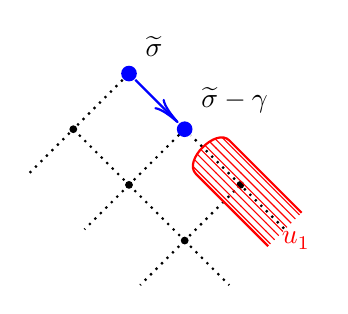
\begin{tikzpicture}[thick, scale=1]
\newcommand{\point}[1]{node (#1) [circle,inner sep=1,fill] {}}
\draw[dotted] (0,0) node (sigma) [circle,inner sep=2,fill=blue,label=above right:{$\widetilde\sigma$}] {} ++(-45:1) node (sigmaminusgamma) [circle,inner sep=2,fill=blue,label=above right:{$\widetilde\sigma-\gamma$}] {} -- ++(-90-45:1) \point{} -- ++(90+45:1) \point{} -- +(-90-45:0.8) ++(-45:1) -- +(-90-45:0.8) ++(0:0) -- ++(-45:1) \point{} -- ++(45:1) \point{} -- +(-45:0.8) ++(-90-45:1) -- +(-45:0.8) ++(0:0) -- +(-90-45:0.8) ++(45:1) -- (sigmaminusgamma) (sigma) -- +(-90-45:1);
\draw[blue,-{>[length=10,width=5]}] (sigma) -- (sigmaminusgamma);
\draw[red,pattern=north west lines, pattern color=red] (-45:2.8) ++(45:0.3) -- ++(90+45:1.3) to[bend right=90] ++(-90-45:0.6) -- ++(-45:1.3) ++(45:0.3);
\node[red] at (-45:3.0) {$u_1$};
\end{tikzpicture}
\end{center}

\begin{multline*}
h_{-2\gamma} \coloneqq [x_{-\gamma}(1),h_{-\gamma}] = \\ =
[x_{-\gamma}(1), x_{\beta-\gamma}(N_{-\gamma,\beta,1,1} \,\xi) \, x_{\beta-2\gamma}(\ldots) \, \varepsilon_{-\gamma}(u) \, u_1] = \\ =
[x_{-\gamma}(1), x_{\beta-\gamma}(N_{-\gamma,\beta,1,1} \,\xi) \, x_{\beta-2\gamma}(\ldots)] \cdot \\ \cdot {}^{x_{\beta-\gamma}(N_{-\gamma,\beta,1,1} \,\xi) \, x_{\beta-2\gamma}(\ldots)} [x_{-\gamma}(1), \varepsilon_{-\gamma}(u) \, u_1] = \\ =
x_{\beta-2\gamma}(N_{-\gamma,\beta,1,1} N_{-\gamma,\beta-\gamma,1,1} \, \xi) \; \varepsilon^2_{-\gamma}(u) \, u_2 \; ,
\end{multline*}
где $u_2$ раскладывается по подпространствам $U_\sigma$ с $\sigma \in \widetilde\sigma-2\gamma - \N \, \gamma$.

\begin{center}
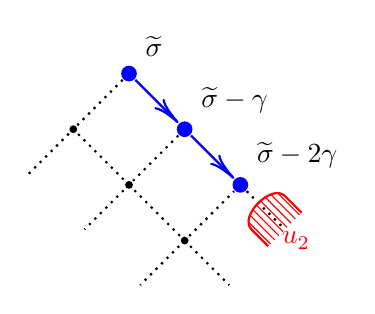
\begin{tikzpicture}[thick, scale=1]
\newcommand{\point}[1]{node (#1) [circle,inner sep=1,fill] {}}
\draw[dotted] (0,0) node (sigma) [circle,inner sep=2,fill=blue,label=above right:{$\widetilde\sigma$}] {} ++(-45:1) node (sigmaminusgamma) [circle,inner sep=2,fill=blue,label=above right:{$\widetilde\sigma-\gamma$}] {} ++(-45:1) node (sigmaminus2gamma) [circle,inner sep=2,fill=blue,label=above right:{$\widetilde\sigma-2\gamma$}] {} (sigmaminusgamma) -- ++(-90-45:1) \point{} -- ++(90+45:1) \point{} -- +(-90-45:0.8) ++(-45:1) -- +(-90-45:0.8) ++(0:0) -- ++(-45:1) \point{} -- (sigmaminus2gamma) -- +(-45:0.8) ++(-90-45:1) -- +(-45:0.8) ++(0:0) -- +(-90-45:0.8) (sigma) -- +(-90-45:1);
\draw[blue,-{>[length=10,width=5]}] (sigma) -- (sigmaminusgamma);
\draw[blue,-{>[length=10,width=5]}] (sigmaminusgamma) -- (sigmaminus2gamma);
\draw[red,pattern=north west lines, pattern color=red] (-45:2.8) ++(45:0.3) -- ++(90+45:0.3) to[bend right=90] ++(-90-45:0.6) -- ++(-45:0.3) ++(45:0.3);
\node[red] at (-45:3.0) {$u_2$};
\end{tikzpicture}
\end{center}

Аналогично вводятся $h_{-\delta}$ и $h_{-2\delta}$, а также $h_{-3\gamma}$ и $h_{-3\delta}$.
\begin{multline*}
h_{-3\gamma} \coloneqq [x_{-\gamma}(1),h_{-2\gamma}] = \\ =
[x_{-\gamma}(1), x_{\beta-2\gamma}(N_{-\gamma,\beta,1,1} N_{-\gamma,\beta-\gamma,1,1} \, \xi) \; \varepsilon^2_{-\gamma}(u) \, u_2] = \\ =
{}^{x_{\beta-2\gamma}(N_{-\gamma,\beta,1,1} N_{-\gamma,\beta-\gamma,1,1} \, \xi)}[x_{-\gamma}(1),\varepsilon^2_{-\gamma}(u) \, u_2] =
\varepsilon^3_{-\gamma}(u) \, u_3
 \; ,
\end{multline*}
где $u_3$ раскладывается по подпространствам $U_\sigma$ с $\sigma \in \widetilde\sigma-3\gamma - \N \, \gamma$.

Вернёмся к разбору вариантов леммы \ref{highestweightvariants}.
\begin{itemize}
\item Если угол между $\gamma$ и $\delta$ составляет $\frac{2\pi}{3}$:
\begin{enumerate}
\item $ \sigma - \gamma \notin \Sigma$, тогда $h_{-\gamma}=x_{\beta-\gamma}(N_{-\gamma,\beta,1,1} \,\xi)\in E\cap H$ и $x_\beta(\xi)\in H$
\item $ \sigma - \delta \notin \Sigma$, тогда $h_{-\delta}=x_{\beta-\delta}(N_{-\delta,\beta,1,1} \,\xi)\in E\cap H$ и $x_\beta(\xi)\in H$
\item $ \sigma - 2\gamma \in \Sigma$, тогда $h_{-2\gamma}=\varepsilon_{-\gamma}^2(u)\in U\cap H$ и по \ref{extremalweightisomorphism} $u\in H$
\item $ \sigma - 2\delta \in \Sigma$, тогда $h_{-2\delta}=\varepsilon_{-\delta}^2(u)\in U\cap H$ и по \ref{extremalweightisomorphism} $u\in H$
\end{enumerate}
\item Если угол между $\gamma$ и $\delta$ составляет $\frac{\pi}{2}$:
\begin{enumerate}
\item[0.] $ \sigma - \delta + \gamma \in \Sigma$ --- случай разобран ранее
\item $ \sigma - 2\gamma \notin \Sigma$, тогда $h_{-2\gamma}=x_{\beta-2\gamma}(N_{-\gamma,\beta,1,1}N_{-\gamma,\beta-\gamma,1,1} \,\xi)\in E\cap H$ и $x_\beta(\xi)\in H$
\item $ \sigma - 2\delta \notin \Sigma$, тогда $h_{-2\delta}=x_{\beta-2\delta}(N_{-\delta,\beta,1,1}N_{-\delta,\beta-\delta,1,1} \,\xi)\in E\cap H$ и $x_\beta(\xi)\in H$
\item $ \sigma - 3\gamma \in \Sigma$, тогда $h_{-3\gamma}=\varepsilon_{-\gamma}^3(u)\in U\cap H$ и по \ref{extremalweightisomorphism} $u\in H$
\item $ \sigma - 3\delta \in \Sigma$, тогда $h_{-3\delta}=\varepsilon_{-\delta}^3(u)\in U\cap H$ и по \ref{extremalweightisomorphism} $u\in H$
\end{enumerate}
\end{itemize}
\end{proof}

\begin{thm}
В условиях предыдущей теоремы подгруппа $H\le G \rightthreetimes U$ может быть представлена в виде $H = H_G \rightthreetimes H_U$, где $[H_G,E] = \prod_{i=1}^n E(\Phi_i, R, I_i)$, а $H_U=U_I$ --- подмодуль $U$, заданный некоторым идеалом кольца.
\end{thm}
\begin{proof}
Достаточно доказать, что $H_G \le H$, оставшаяся часть формулировки взята из \ref{unipotenttransitivity}.

Разложим элемент $h \in H$ в произведение $h = z u$, где $z \in H_G$, $u \in U$. Докажем, что $z$ и $u$ также лежат в $H$.

Прокоммутируем $h$ с некоторым $g$ из $E$:
$$ [g, h] = [g,zu] = [g,z] \cdot {}^z[g,u] $$

По теореме \ref{subgroupprojectionmain} $[g,z]\in H$, следовательно, ${}^z[g,u]$ так же лежит в $H$. Но
$ {}^z[g,u] = {}^{zu}[u^{-1},g] $, следовательно, $[u^{-1},g] \in H$. Выбирая в качестве $g$ корневые элементы $x_\alpha(1)$ с корнями из начала цепочек в лемме \ref{returnfromhighest}, получим, что $u$ также лежит в $H$.
\end{proof}

\section{Случай присоединённого представления}

Описанный выше результат о виде подгрупп, нормализуемых $E$, получен при выполнении предположений теоремы \ref{subgroupprojectionmain}. Среди этих условий выделяется условие о том, что все $\widetilde\sigma-\widetilde\beta_i$ не ортогональны соответствующим $\Phi_i$. Это требование вытекает из леммы \ref{maxrootsum} и отделяет случай, когда для некоторого $\Phi_i$ оказывается $\widetilde\sigma-\widetilde\beta_i$ ортогонально $\Phi_i$. Этот случай является существенным исключением, и для него выполняется более слабый результат.

\begin{prop}
Пусть выполняются условия теоремы \ref{subgroupprojectionmain} за исключением требования $\widetilde\sigma-\widetilde\beta_i \not\perp \Phi_i \; \forall i$. А именно, пусть для некоторого $i$ выполнено $\widetilde\sigma-\widetilde\beta_i \perp \Phi_i$.

Тогда если $x_{\widetilde\beta_i}(\xi) \in H_G$, то $x_{\widetilde\beta_i}(\xi^2) \in H$.
\end{prop}
\begin{proof}
\# Верно ли, если в $\Phi_i$ не содержится $A_2$? Тогда там содержится $B_2$ --- провести вычисления.
\end{proof}

\section{Обобщение на случай неабелева унипотентного радикала}

Группы, рассмотренные выше, являются нередуктивными линейными алгебраическими группами с абелевым унипотентным радикалом.

Перейдём теперь к рассмотрению групп, получающихся подобным же образом из представлений, но в которых унипонетный радикал будет уже не абелев, в класса нильпотентности 2, то есть коммутант унипотентного радикала будет абелевым.

\begin{tcolorbox}[colback=white]
\begin{definition}
Пусть $U$ --- $G$-модуль, являющийся алгеброй над $R$ с умножением, которое согласовано с действием $G$:
$$\circledast : U \times U \to U$$
$$ {}^g u \circledast {}^g v = {}^g (u \circledast v) .$$

При этом, обозначив $V:=U\circledast U$, будем предполагать, что $U$ раскладывается в прямую сумму $U = U/V \oplus V$.

Тогда можно рассмотреть группу $P$, являющуюся расширением $G$ с помощью $U$, элементами которой будут пары $(g,u)$, $g \in G$, $u \in U$ со следующим умножением:
$$
(g,u)\cdot (g',u') = (g g', {}^{g'^{-1}} u + u' + {}^{g'^{-1}} u \circledast u')
$$

Такая группа называется \textit{\textbf{параболически-сходной группой с унипотентным радикалом класса нильпотентности 2}}.
\end{definition}
\end{tcolorbox}

\begin{tcolorbox}[colback=white]
\begin{example}
Если $V=0$, то есть $u \circledast u'$ всегда тривиально, то эта конструкция представляет собой полупрямое произведение группы $G$ и аддитивной группы модуля $U$.
\end{example}
\end{tcolorbox}

Если же $u \circledast u'$ нетривиально, то $P$ тоже является полупрямым произведением группы $G$ и группы, состоящей из элементов из $U$ с умножением
$
(u,u') \mapsto u + u' + u \circledast u'
$.

\begin{example}
Частным случаем предыдущего примера является пример, когда группа $G$ является прямым произведением групп $G_1,\ldots ,G_n$, а модуль $U$ раскладывается в прямую сумму $U_1 \oplus \ldots \oplus U_{n-1}$ со следующими действиями групп на них:
\begin{equation*}
\begin{array}{lcccr}
G_1 & \lacts & U_1 & \racts & G_2 \\
\hdotsfor{5}\\
G_{n-1} & \lacts & U_{n-1} & \racts & G_n
\end{array}
\end{equation*}

Тогда действие $G$ на $U$ конструируется из левых и правых действий $G_1\ldots G_n$ следующим образом:
\begin{equation*}
(g_1,\ldots , g_n) : u_i \mapsto g_i u_i g_{i+1}^{-1}
\end{equation*}


В результате $P = G \rightthreetimes U$ можно записать как факторгруппу группы матриц вида
\begin{equation*}
\begin{pmatrix}
g_1 & g_1 u_1 &     &     & \bigzero{*}{-2} \\
    & g_2 & g_2 u_2 & &  \\
    &    &\ddots&\ddots&    \\
    &     &     &g_{n-1}& g_{n-1} u_{n-1} \\
\bigzero{0}{3}& &     &     & g_n \\
\end{pmatrix}
\end{equation*}

по подгруппе вида
\begin{equation*}
\begin{pmatrix}
1 & 0 &      &      & \bigzero{*}{-2} \\
  & 1 & 0    &      &   \\
  &   &\ddots&\ddots&   \\
  &   &      &1     & 0 \\
\bigzero{0}{3}&&&   & 1 \\
\end{pmatrix}
\end{equation*}
\end{example}

\begin{example}
Обобщая предыдущий пример на случай $V\neq0$, можно рассмотреть факторгруппу матриц вида
\begin{equation*}
\resizebox{.9\hsize}{!}{$
\left.
\begin{pmatrix}
g_1 & g_1 u_1 & g_1 v_1 &      & &  & \bigzero{*}{-1}        \\
    & g_2     & g_2 u_2 & \ddots &    &  &  \\
    &         & g_3     & \ddots  & \ddots &  &    \\
    &         &         & \ddots  & \ddots & \ddots  &    \\
    &      &  & & g_{n-2}     & g_{n-2} u_{n-2} & g_{n-2} v_{n-2} \\
    &      &  & &         & g_{n-1}     & g_{n-1} u_{n-1} \\
\bigzero{0}{3} & &  &  &    &         & g_n     \\
\end{pmatrix}
\right/
\begin{pmatrix}
  1 &       0 & 0       &        & \bigzero{*}{-1}  \\
    & \ddots  & \ddots  & \ddots &                  \\
    &         & 1       & 0      & 0                \\
    &         &         & 1      & 0                \\
\bigzero{0}{3} & &      &        & 1                \\ 
\end{pmatrix}
$},
\end{equation*}

где
\begin{equation*}
\resizebox{.9\hsize}{!}{$
\begin{array}{lcccr}
G_1 & \lacts & U_1 & \racts & G_2 \\
\hdotsfor{5}\\
G_{n-1} & \lacts & U_{n-1} & \racts & G_n\\
\vspace{3ex}\\
G_1 & \lacts & V_1 & \racts & G_3 \\
\hdotsfor{5}\\
G_{n-2} & \lacts & V_{n-2} & \racts & G_n
\end{array}
$
\qquad
$
\begin{array}{lcccr}
\circledast & : & U_1 \times U_2 & \to & V_1 \\
\hdotsfor{5}\\
\circledast & : & U_{n-2} \times U_{n-1} & \to & V_{n-2}
\end{array}
$}
\end{equation*}

При этом согласованность операции $\circledast$ с действиями групп означает, что
\begin{multline*}
(g_1 u_1 g_2^{-1}, \ldots, g_{n-1} u_{n-1} g_n^{-1}) \circledast (g_1 u'_1 g_2^{-1}, \ldots, g_{n-1} u'_{n-1} g_n^{-1}) 
= \\ =
(g_1 u_1 g_2^{-1} g_2 u'_2 g_3^{-1}, \ldots) = 
(g_1 u_1 u'_2 {g}_3^{-1}, \ldots, g_{n-2} u_{n-2} u'_{n-1} g_n^{-1}).
\end{multline*}
\end{example}

\begin{tcolorbox}[colback=white]
\begin{example}
Чтобы группа $P$ была похожа на параболические подгруппы, нужно дополнительно потребовать, чтобы $U \circledast V = V \circledast U = 0$, то есть чтобы
$$ \circledast : U/V \times U/V \to V.$$

Тогда результирующая группа будет состоять из троек $(g,u,v)$, $g \in G$, $u \in U/V$, $v \in V$ со следующим умножением:
$$
(g,u,v)\cdot (g',u',v') = (g g', {}^{g'^{-1}} u + u', {}^{g'^{-1}} v + v' + {}^{g'^{-1}} u \circledast u').
$$
\end{example}
\end{tcolorbox}

\begin{thm}
Пусть $P$ --- параболически-сходная группа над $R$ с унипотентным радикалом класса 2, построенная по представлению $U$ группы $G$ со структурой алгебры~${\circledast}$ на представлении, причём  $U=V \oplus U/V$, где $V:=U\circledast U$.

Тогда если $V$ и $U/V$ --- простые представления группы $G$, для которых с учётом выбора кольца $R$ выполняется свойство \ref{returnfromhighest}, то подгруппы унипотентного радикала, нормализуемые $E$, задаются парой идеалов $I$, $J$, где $I^2 \subset J$.
\end{thm}
\begin{proof}
Пусть $U'\le U$ --- подгруппа, нормализуемая $E$. Так как $P$ допускает факторизацию по $V$, то в $U/V$ будет подгруппа $U'/V$, так же нормализуемая $E$. Аналогично, в $V$ есть подгруппа $U' \cap V$, нормализуемая $E$. А так как $E$-инвариантные подмодули в $U/V$ и в $V$ определяются утверждением \ref{unipotentsubgroups}, то осталось доказать, что $I^2 \subset J$. Но это следует из замкнутости подмодуля относительно~${\circledast}$.
\end{proof}

Если $V$ и $U/V$ --- простые представления, то они раскладываются по весовым пространствам. Следующая лемма говорит о том, что операция~${\circledast}$ согласована с весовым разложением.

\begin{lm}
Если $u,u' \in U/V$ --- векторы весов $\sigma, \sigma'$, то $u \circledast u' \in V$ --- вектор веса $\sigma + \sigma'$.
\end{lm}
\begin{proof}
$$
{}^h(u \circledast u') = {}^h u  \circledast {}^h u' = \sigma(h) u \; \circledast \; \sigma'(h) u' = \sigma(h)\sigma'(h) \enspace u \circledast u'
$$
\end{proof}

Наличие согласованного с действием $G$ весового разложения позволяет предположить, что для параболически-сходных групп с унипотентным радикалом класса нильпотентности~2 может быть получен результат, аналогичный теореме \ref{subgroupprojectionmain}.

\section{Заключение}

\placeholder

\setmonofont[Mapping=tex-text]{CMU Typewriter Text}
\bibliographystyle{ugost2008ls}
\bibliography{references.bib}
\end{document}

